
\chapter{The Legendre Transform}
\label{ch:lt}
The Legendre transform replaces a function by a description in terms of its
\emph{slope}. It is the mathematical engine behind the passage from the
Lagrangian to the Hamiltonian formulation of mechanics, behind the family of
thermodynamic potentials, behind convex duality in optimization, and behind
the large-deviation description of statistical fluctuations.  This article
develops the transform from first principles.  We start with the smooth
one-dimensional case and explain \emph{why} the definition has the form it
has, give its geometric meaning (tangent intercepts, envelopes, areas under
the curve), prove its main properties, and extend it to several variables and
to partial transforms.  We then pass to the Legendre--Fenchel transform of
convex analysis, which removes all smoothness and invertibility assumptions
and explains what happens for non-differentiable and non-convex functions.
A catalogue of worked examples is followed by applications to classical
mechanics, thermodynamics, statistical mechanics and large deviations, a
short section on numerical computation, and remarks on the geometric
background and on generalisations.

\section{Introduction}
% =================================================================

Suppose a physical or mathematical quantity is described by a function
$y=f(x)$, and that the \emph{derivative} $p=f'(x)$ is the variable that we can
actually control, measure, or that is conserved.  In mechanics, $x$ is a
velocity and $p$ a momentum; in thermodynamics, $x$ is an entropy and $p$ a
temperature; in optimization, $x$ is a primal variable and $p$ a Lagrange
multiplier or price.  The question is: can we trade $x$ for $p$ as the
independent variable \emph{without losing any information}?

The Legendre transform is the answer.  It maps a function $f$ of $x$ to a
function $f^*$ of $p=f'(x)$ in such a way that
\begin{itemize}[nosep]
  \item $f$ can be reconstructed from $f^*$ (the transform is an involution
        for convex functions),
  \item the roles of the variable and the derivative are exchanged:
        $f'=(f^*{}')^{-1}$,
  \item the transform is characterised by a variational principle,
        $f^*(p)=\sup_x\,[\,px-f(x)\,]$, which makes sense far beyond the
        smooth setting.
\end{itemize}

\paragraph{Conventions and names.}
We use $f^*(p)=\sup_x[px-f(x)]$.  This object is called the
\emph{Legendre transform} when $f$ is smooth and strictly convex, and the
\emph{Legendre--Fenchel transform} or \emph{convex conjugate} in general.
Physicists often use the opposite sign, $f(x)-px$ evaluated at the stationary
point (for instance $F=U-TS$ in thermodynamics, which equals $-U^*(T)$); we
will point out each such sign when it matters.
\section{The one-dimensional smooth case}\label{sec:1d}
% =================================================================

\subsection{The problem the transform solves}

Let $f$ be smooth with $f''>0$ on an interval $I$.  Then the slope
$p=f'(x)$ is a strictly increasing function of $x$, hence invertible:
$x=x(p)$.  The most naive way to ``use $p$ as the independent variable'' is
to define
\[
  g(p):=f\bigl(x(p)\bigr).
\]
This \emph{loses information}.  Take the family of translates
$f_a(x)=\tfrac12(x-a)^2$.  Then $f_a'(x)=x-a$, so $x(p)=p+a$ and
$g_a(p)=\tfrac12 p^2$ for every $a$: all the curves share the same $g$, yet
they are different functions.  The reason is visible in the chain rule:
$g'(p)=f'(x(p))\,x'(p)=p\,x'(p)$ determines $x(p)$, i.e.\ the inverse of
$f'$, only up to an additive constant, and that constant is precisely the
horizontal position of the curve.

Differently put: the function $g$ stores the curve only up to translation in
$x$.  We need a different quantity that depends on $p$ and that does
determine $f$.

\subsection{Tangent lines and the definition}

The tangent line to the graph of $f$ at the point $x$ has slope $p=f'(x)$:
\[
  \ell(\xi)=f(x)+p\,(\xi-x).
\]
Its intercept with the vertical axis ($\xi=0$) is
\[
  b = f(x)-p\,x .
\]
A curve is determined by the family of its tangent lines, and a tangent line
is determined by the pair (slope, intercept).  Recording the intercept as a
function of the slope, $b=b(p)$, therefore keeps all the information.  The
Legendre transform is $f^*=-b$; the sign is chosen so that $f^*$ is again
convex.

\begin{definition}[Legendre transform, smooth case]\label{def:legendre1d}
Let $I\subseteq\mathbb{R}$ be an open interval and $f\in C^2(I)$ with $f''>0$ on
$I$.  Then $f'\colon I\to J:=f'(I)$ is a $C^1$-diffeomorphism onto an open
interval $J$ (monotonicity, continuity, and the inverse function theorem).
Write $x(p):=(f')^{-1}(p)$. The \emph{Legendre transform} of $f$ is
\[
  f^*(p) := p\,x(p)-f\bigl(x(p)\bigr),\qquad p\in J .
\]
\end{definition}

\subsection{Basic properties}

\begin{proposition}\label{prop:basic1d}
With the notation of Definition~\ref{def:legendre1d}:
\begin{enumerate}[label=(\alph*),nosep]
  \item $f^*\in C^2(J)$ and $(f^*)'(p)=x(p)$.
  \item $(f^*)''(p)=1/f''\bigl(x(p)\bigr)>0$.
  \item (Variational characterisation) $f^*(p)=\max_{\xi\in I}\,[\,p\xi-f(\xi)\,]$,
        and the maximum is attained only at $\xi=x(p)$.
  \item (Fenchel--Young inequality) $f(x)+f^*(p)\ge px$ for all $x\in I$,
        $p\in J$, with equality if and only if $p=f'(x)$.
  \item (Involution) $(f^*)^*=f$.
\end{enumerate}
\end{proposition}

\begin{proof}
(a) Since $x(\cdot)$ is $C^1$, so is $f^*$, and by the product and chain rules
\[
  (f^*)'(p)=x(p)+p\,x'(p)-f'\bigl(x(p)\bigr)\,x'(p)
          =x(p)+\bigl(p-f'(x(p))\bigr)x'(p)=x(p),
\]
because $f'(x(p))=p$.  Thus $(f^*)'=x(\cdot)$ is again $C^1$, so
$f^*\in C^2$.

(b) Differentiating the identity $f'(x(p))=p$ gives
$f''(x(p))\,x'(p)=1$, i.e.\ $x'(p)=1/f''(x(p))$.  By (a) this is
$(f^*)''(p)$.

(c) Fix $p\in J$ and let $\varphi(\xi)=p\xi-f(\xi)$.  Then
$\varphi''=-f''<0$, so $\varphi$ is strictly concave, and
$\varphi'(\xi)=p-f'(\xi)$ vanishes exactly at $\xi=x(p)$.  A strictly
concave function attains its global maximum exactly at its critical point;
the maximum value is $\varphi(x(p))=f^*(p)$.

(d) By (c), $f^*(p)\ge p\xi-f(\xi)$ for every $\xi\in I$, with equality iff
$\xi=x(p)$, i.e.\ iff $p=f'(\xi)$.

(e) By (a) and (b), $f^*$ satisfies the hypotheses of
Definition~\ref{def:legendre1d} on $J$, and its derivative
$(f^*)'=x(\cdot)\colon J\to I$ has inverse $f'$.  Hence
\[
  (f^*)^*(x)=x\,p(x)-f^*\bigl(p(x)\bigr),\qquad p(x)=f'(x),
\]
and inserting $f^*(p(x))=p(x)\,x-f(x)$ gives
$(f^*)^*(x)=x f'(x)-\bigl[f'(x)\,x-f(x)\bigr]=f(x)$.
\end{proof}

Property (a) is the heart of the matter: \emph{the derivative of $f^*$ is the
inverse function of the derivative of $f$}.  The two functions $f'$ and
$(f^*)'$ undo each other, which is why $f^*$ contains the same information as
$f$.  Property (b) says that curvatures are reciprocal:
\[
  f''(x)\,(f^*)''(p)=1\qquad\text{whenever } p=f'(x).
\]
Sharply curved functions have flatly curved transforms and vice versa.

% ----------------------------------------------------------------
\subsection{Geometric interpretation}\label{sec:geometry}
% ----------------------------------------------------------------

\paragraph{(i) Intercepts of tangents.}
By construction, $-f^*(p)$ is the vertical intercept of the tangent line of
slope $p$ (Figure~\ref{fig:tangent}).

\begin{figure}[ht]
\centering
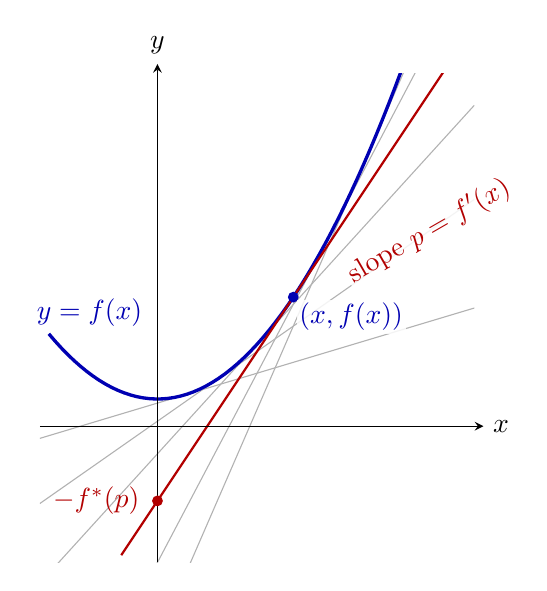
\begin{tikzpicture}[scale=1.15,>=stealth]
  \begin{scope}
    \clip (-1.3,-1.5) rectangle (3.5,3.9);
    % family of tangent lines to y = x^2/2 + 0.3
    \foreach \a in {0.3,0.7,1.1,1.9,2.3} {
      \draw[gray!60,thin,domain=-1.3:3.5] plot (\x,{\a*\x-\a*\a/2+0.3});
    }
    % the curve
    \draw[very thick,blue!70!black,domain=-1.2:2.9,samples=60] plot (\x,{0.5*\x*\x+0.3});
    % highlighted tangent, slope p = 1.5, intercept -0.825
    \draw[thick,red!70!black,domain=-0.4:3.5] plot (\x,{1.5*\x-0.825});
  \end{scope}
  \draw[->] (-1.3,0) -- (3.6,0) node[right] {$x$};
  \draw[->] (0,-1.5) -- (0,4.0) node[above] {$y$};
  \fill[red!70!black] (0,-0.825) circle (1.7pt);
  \node[left=3pt,red!70!black] at (0,-0.825) {$-f^*(p)$};
  \fill[blue!70!black] (1.5,1.425) circle (1.7pt);
  \node[below right=1pt,blue!70!black,fill=white,fill opacity=0.85,text opacity=1,inner sep=1pt] at (1.5,1.425) {$(x,f(x))$};
  \node[blue!70!black] at (-0.75,1.25) {$y=f(x)$};
  \node[red!70!black,rotate=30,fill=white,fill opacity=0.85,text opacity=1,inner sep=1pt] at (3.0,2.15) {slope $p=f'(x)$};
\end{tikzpicture}
\caption{The curve $y=f(x)$ (blue), some of its tangent lines (grey), and the
tangent of slope $p$ (red).  Its vertical intercept is $f(x)-px=-f^*(p)$.  The
curve is the \emph{envelope} of the lines $y=p\xi-f^*(p)$.}
\label{fig:tangent}
\end{figure}

\paragraph{(ii) Envelope of a family of lines.}
The tangent line of slope $p$ is $y=p\xi-f^*(p)$.  A curve is the envelope of
a one-parameter family $F(\xi,y,p)=0$ if it is the set of points that satisfy
$F=0$ and $\partial F/\partial p=0$.  Here $F=p\xi-f^*(p)-y$, so
\[
  0=\pd{F}{p}=\xi-(f^*)'(p)\ \Longrightarrow\ \xi=x(p),\qquad
  y=p\,x(p)-f^*(p)=f\bigl(x(p)\bigr).
\]
Thus the graph of $f$ is recovered as the envelope of the lines whose
slopes and intercepts are given by $f^*$.  This is the geometric content of
$(f^*)^*=f$ and shows that point-wise and line-wise descriptions of a curve
are dual to each other.

\paragraph{(iii) Areas in the phase plane.}
Consider the curve $\Gamma=\{(x,p):p=f'(x)\}$ in the $(x,p)$-plane.  Read as
a graph over $x$, it gives $f$ by integration,
$f(x)=f(x_0)+\int_{x_0}^{x}p\,d x'$; read as a graph over $p$ it gives
\[
  f^*(p)=f^*(p_0)+\int_{p_0}^{p}x\,d p' .
\]
(The second formula is $(f^*)'=x$.)  \emph{The two functions are the two
integrals of the same curve}, one along each axis.  Normalise $f(0)=f'(0)=0$.
Then $f(x)$ is the area under $\Gamma$ and $f^*(p)$ is the area to its left
(Figure~\ref{fig:areas}), and together they fill the rectangle $[0,x]\times[0,p]$:
\[
  f(x)+f^*(p)=xp\qquad\text{for }(x,p)\in\Gamma,
\]
which is integration by parts.  For a point $(x,p)$ \emph{off} the curve the
two regions still cover the rectangle, but one of them extends beyond it, so
$f(x)+f^*(p)\ge xp$---the Fenchel--Young inequality (d) of
Proposition~\ref{prop:basic1d}.

\begin{figure}[ht]
\centering
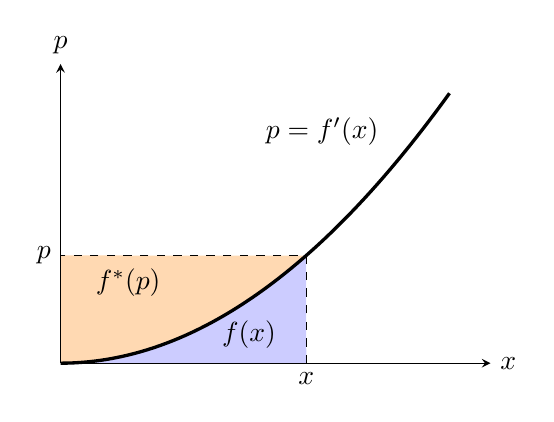
\begin{tikzpicture}[x=2.6cm,y=0.95cm,>=stealth]
  \fill[blue!20] (0,0) -- plot[domain=0:1.2,samples=50,variable=\t] ({\t},{\t*\t}) -- (1.2,0) -- cycle;
  \fill[orange!30] (0,0) -- plot[domain=0:1.2,samples=50,variable=\t] ({\t},{\t*\t}) -- (0,1.44) -- cycle;
  \draw[->] (0,0) -- (2.1,0) node[right] {$x$};
  \draw[->] (0,0) -- (0,4.0) node[above] {$p$};
  \draw[very thick,domain=0:1.9,samples=60,variable=\t] plot ({\t},{\t*\t});
  \draw[dashed] (1.2,0) -- (1.2,1.44) -- (0,1.44);
  \node[below] at (1.2,0) {$x$};
  \node[left] at (0,1.44) {$p$};
  \node at (0.92,0.38) {$f(x)$};
  \node at (0.33,1.08) {$f^*(p)$};
  \node[left] at (1.6,3.1) {$p=f'(x)$};
\end{tikzpicture}
\caption{For $f(x)=x^3/3$ (so $p=x^2$ and $f^*(p)=\tfrac23p^{3/2}$): $f(x)$ is
the area under the curve (blue), $f^*(p)$ the area to its left (orange), and
together they make up the rectangle of area $xp$.}
\label{fig:areas}
\end{figure}

\paragraph{(iv) Contact-geometric formulation.}
Consider the space of triples $(x,y,p)$ with the contact form
$\alpha=d y-p\,d x$.  The \emph{1-jet} of $f$, the curve
$x\mapsto(x,f(x),f'(x))$, is exactly a curve along which $\alpha=0$.  The map
\[
  (x,y,p)\longmapsto (X,Y,P)=(p,\;px-y,\;x)
\]
satisfies $d Y-P\,d X=p\,d x+x\,d p-d y-x\,d p=-\alpha$, so it
preserves the contact structure, and it sends the 1-jet of $f$ to the 1-jet of
$Y=f^*(X)$.  The Legendre transform is thus a \emph{contact transformation};
the same statement in the cotangent bundle is the symplectic structure
underlying Hamiltonian mechanics (Section~\ref{sec:remarks}).

\begin{remark}[Why not just invert?]
The equivalent descriptions of a convex curve are: points $(x,f(x))$,
slopes $p(x)$, tangent intercepts $-f^*(p)$.  Only the first and third
determine the curve.  The slope function alone does not, and neither does
$f(x(p))$, because they forget a horizontal translation.  Thermodynamic
analogue: knowing the internal energy as a function of temperature,
$U=\tfrac32NkT$, does not determine the pressure of an ideal gas,
whereas the free energy $F(T,V,N)$ does (Section~\ref{sec:thermo}).
\end{remark}

% =================================================================
\section{Several variables}\label{sec:nd}
% =================================================================

\subsection{The smooth strictly convex case}

\begin{theorem}\label{thm:nd}
Let $\Omega\subseteq\mathbb{R}^n$ be open and convex, and let $f\in C^2(\Omega)$ have
positive definite Hessian at every point.  Then:
\begin{enumerate}[label=(\roman*),nosep]
  \item $\nabla f\colon\Omega\to\Omega^*:=\nabla f(\Omega)$ is a
        $C^1$-diffeomorphism onto an open set $\Omega^*$.  Write
        $x(p)=(\nabla f)^{-1}(p)$.
  \item The function $f^*(p):=\ip{p}{x(p)}-f(x(p))$ on $\Omega^*$ satisfies
        $f^*(p)=\max_{\xi\in\Omega}\,[\ip{p}{\xi}-f(\xi)]$.
  \item $\nabla f^*=(\nabla f)^{-1}$ and
        $\Hess f^*(p)=\bigl[\Hess f(x(p))\bigr]^{-1}$ (in particular, it is
        positive definite).
  \item $f^{**}=f$ on $\Omega$, and $f(x)+f^*(p)\ge\ip{p}{x}$ with equality iff
        $p=\nabla f(x)$.
\end{enumerate}
\end{theorem}

\begin{proof}
(i) \emph{Injectivity.} Suppose $x\neq y$ in $\Omega$ and put $v=y-x$,
$g(t)=\ip{\nabla f(x+tv)}{v}$ for $t\in[0,1]$ (the segment lies in $\Omega$ by
convexity).  Then $g'(t)=v^{\mathsf T}\Hess f(x+tv)\,v>0$, so
$g(0)\neq g(1)$ and hence $\nabla f(x)\neq\nabla f(y)$.  \emph{Local
diffeomorphism.} The Jacobian of $\nabla f$ is $\Hess f$, which is
invertible, so the inverse function theorem applies; in particular $\nabla f$
is an open map and $\Omega^*$ is open.

(ii) For fixed $p\in\Omega^*$, $\varphi(\xi)=\ip{p}{\xi}-f(\xi)$ is strictly
concave on the convex set $\Omega$ with $\nabla\varphi(\xi)=p-\nabla f(\xi)=0$ at
$\xi=x(p)$; hence this is the unique global maximiser.

(iii) In indices, using $\partial_jf(x(p))=p_j$,
\[
  \pd{f^*}{p_i}=x_i+\sum_j\bigl(p_j-\partial_jf(x(p))\bigr)\pd{x_j}{p_i}=x_i .
\]
Differentiating $\nabla f(x(p))=p$ gives
$\Hess f(x(p))\,Dx(p)=\mathbb 1$, so $Dx=(\Hess f)^{-1}$, and
$\Hess f^*=D(\nabla f^*)=Dx$.

(iv) $\nabla f^*\colon\Omega^*\to\Omega$ is the inverse of $\nabla f$, so
by (iii) $f^*$ satisfies the hypotheses on $\Omega^*$ (locally; the argument
for $f^{**}$ only uses the formula and the bijection), and
$f^{**}(x)=\ip{x}{p(x)}-f^*(p(x))=\ip{x}{\nabla f(x)}-[\ip{\nabla f(x)}{x}-f(x)]=f(x)$.
Fenchel--Young follows from (ii) as in the one-dimensional case.
\end{proof}

\subsection{Partial Legendre transforms}

In applications one often transforms with respect to \emph{some} variables
and keeps the others as passive parameters.  Let $f=f(x,y)$ with
$x\in\mathbb{R}^m$, $y\in\mathbb{R}^\ell$, and $\Hess_xf\succ0$.  Define
\[
  g(p,y):=\sup_{x}\,\bigl[\ip{p}{x}-f(x,y)\bigr]=\ip{p}{x(p,y)}-f\bigl(x(p,y),y\bigr),
  \qquad \pd{f}{x}\bigl(x(p,y),y\bigr)=p .
\]

\begin{proposition}\label{prop:partial}
$\displaystyle \pd{g}{p}=x,\qquad
 \pd{g}{y}\bigg|_{p}=-\pd{f}{y}\bigg|_{x}$.
\end{proposition}

\begin{proof}
Using $\partial_xf=p$,
$\partial_yg=\bigl(p-\partial_xf\bigr)\,\partial_yx-\partial_yf=-\partial_yf$.
The first identity is proved as in Theorem~\ref{thm:nd}(iii).
\end{proof}

The second identity---\emph{derivatives with respect to the passive variables
change sign but are otherwise unchanged}---is what produces Hamilton's
equations in Section~\ref{sec:mech} and the Maxwell relations in
Section~\ref{sec:thermo}.  If only the velocities belonging to ``cyclic''
coordinates are transformed, one obtains the Routhian of classical mechanics.

\subsection{The quadratic case}

For a positive definite symmetric matrix $A$,
\[
  f(x)=\tfrac12\,x^{\mathsf T}Ax+b^{\mathsf T}x+c
  \quad\Longrightarrow\quad
  f^*(p)=\tfrac12\,(p-b)^{\mathsf T}A^{-1}(p-b)-c .
\]
Indeed $\nabla f=Ax+b=p$ gives $x=A^{-1}(p-b)$, and then
$px-f=(p-b)^{\mathsf T}x-\tfrac12x^{\mathsf T}Ax-c=\tfrac12(p-b)^{\mathsf T}A^{-1}(p-b)-c$.
The Hessians $A$ and $A^{-1}$ are inverse to each other, as predicted by
Theorem~\ref{thm:nd}(iii).

% =================================================================
\section{The Legendre--Fenchel transform}\label{sec:fenchel}
% =================================================================

The definition via $x(p)$ requires $f$ to be $C^2$, strictly convex, and its
gradient map to be invertible.  The variational form requires none of this.

\subsection{Definition and first properties}

\begin{definition}[Convex conjugate]
Let $f\colon\mathbb{R}^n\to(-\infty,+\infty]$ be \emph{proper} (not identically
$+\infty$).  Its \emph{Legendre--Fenchel transform} (convex conjugate) is
\[
  f^*(p)=\sup_{x\in\mathbb{R}^n}\,\bigl[\ip{p}{x}-f(x)\bigr]\in(-\infty,+\infty].
\]
\end{definition}

The value $+\infty$ is allowed for $f$ (constraints are encoded as
$f=+\infty$ outside the feasible set) and for $f^*$.

\begin{proposition}\label{prop:fenchelbasic}
For every proper $f$:
\begin{enumerate}[label=(\alph*),nosep]
  \item $f^*$ is convex and lower semicontinuous (it is a pointwise supremum
        of affine functions of $p$), whether or not $f$ is convex.
  \item (Fenchel--Young) $f(x)+f^*(p)\ge\ip{p}{x}$ for all $x,p$.
  \item $f\le g\mathbb{R}ightarrow f^*\ge g^*$ (order reversal), and $f^{**}\le f$.
\end{enumerate}
\end{proposition}

\begin{proof}
(a) For fixed $x$ with $f(x)<\infty$ the map $p\mapsto\ip{p}{x}-f(x)$ is affine,
and $f^*$ is the supremum of these.  (b) is the definition of the supremum.
(c) If $f\le g$ then $\ip{p}{x}-f(x)\ge\ip{p}{x}-g(x)$ for every $x$.  From (b),
$\ip{x}{p}-f^*(p)\le f(x)$ for all $p$; taking the supremum over $p$ gives
$f^{**}\le f$.
\end{proof}

\subsection{The Fenchel--Moreau theorem}

\begin{theorem}[Fenchel--Moreau]\label{thm:fm}
Let $f$ be proper. Then $f^{**}=f$ if and only if $f$ is convex and lower
semicontinuous (``closed'').  More generally, if $f$ has an affine minorant,
$f^{**}$ is the largest closed convex function below $f$, i.e.\ its
\emph{closed convex envelope}; its epigraph is the closure of the convex hull
of $\epi f$.
\end{theorem}

\begin{proof}[Sketch of proof]
By Proposition~\ref{prop:fenchelbasic}(c), $f^{**}\le f$ always.  Suppose $f$
is proper, convex and lower semicontinuous.  Then $\epi f$ is a closed convex
set, and the separating hyperplane theorem shows that $f$ is the pointwise
supremum of its affine minorants.  An affine function
$a(x)=\ip{p}{x}-b$ satisfies $a\le f$ if and only if $b\ge f^*(p)$.  Hence
\[
  f(x)=\sup_{p}\,\bigl[\ip{p}{x}-f^*(p)\bigr]=f^{**}(x).
\]
Conversely $f^{**}$ is a conjugate, hence closed and convex, by
Proposition~\ref{prop:fenchelbasic}(a); so $f=f^{**}$ forces $f$ to be closed
and convex.  For the last statement, if $h\le f$ is closed and convex, then
$h=h^{**}\le f^{**}$ by order reversal.
\end{proof}

\subsection{Subdifferentials: the nonsmooth version of \texorpdfstring{$\nabla f^*=(\nabla f)^{-1}$}{grad f* is the inverse of grad f}}

The \emph{subdifferential} of $f$ at $x$ is
\[
  \partial f(x)=\bigl\{p:\ f(z)\ge f(x)+\ip{p}{z-x}\ \ \forall z\bigr\},
\]
the set of slopes of all affine functions that touch the graph from below at
$x$.

\begin{theorem}\label{thm:subdiff}
For proper $f$: $p\in\partial f(x)\iff f(x)+f^*(p)=\ip{p}{x}$.  If moreover $f$
is closed and convex, these are also equivalent to $x\in\partial f^*(p)$;
that is, $\partial f^*=(\partial f)^{-1}$ as set-valued maps.
\end{theorem}

\begin{proof}
$p\in\partial f(x)$ means $\ip{p}{z}-f(z)\le\ip{p}{x}-f(x)$ for all $z$, i.e.
$f^*(p)=\ip{p}{x}-f(x)$.  Applying this statement to $f^*$ in place of $f$ and
using $f^{**}=f$ (Theorem~\ref{thm:fm}) gives $x\in\partial f^*(p)\iff
f^*(p)+f(x)=\ip{p}{x}$.
\end{proof}

For smooth strictly convex $f$ the subdifferential is the single-valued
gradient and we recover Theorem~\ref{thm:nd}(iii).  In general there is a
dictionary:
\begin{center}
\begin{tabular}{@{}ll@{}}
\toprule
$f$ & $f^*$\\
\midrule
corner (kink) with slopes in $[p_1,p_2]$ & flat piece (affine segment) of slope $x$ over $[p_1,p_2]$\\
flat piece & kink\\
$f=+\infty$ outside a set & $f^*$ grows at most linearly (support function)\\
$f$ superlinear growth & $\dom f^*=\mathbb{R}^n$\\
\bottomrule
\end{tabular}
\end{center}

\subsection{Functions that are not convex}

For a non-convex $f$, the transform $f^*$ is still defined, but it only
``sees'' the closed convex envelope $f^{**}$: $(f^{**})^*=f^*$.
Information about the non-convex parts of $f$ is lost.  Moreover, the
\emph{naive} construction $p\,x-f(x)$ with $f'(x)=p$ becomes multivalued,
because $f'$ is no longer injective.  The sup-definition chooses the
branch with the largest value.

\begin{example}[Double well]\label{ex:doublewell}
Let $f(x)=\tfrac14x^4-\tfrac12x^2$, whose derivative $f'(x)=x^3-x$ is not
monotone.  For $|p|<2/(3\sqrt3)$ the equation $f'(x)=p$ has three real roots.
The function $\varphi(\xi)=p\xi-f(\xi)$ has $\varphi''=1-3\xi^2$, so the
middle root (where $|\xi|<1/\sqrt3$) is a local \emph{minimum} of $\varphi$
and is discarded; the two outer roots are local maxima and compete.  For
$p>0$ the right one wins and for $p<0$ the left one wins.  At $p=0$ the
candidates are $x=\pm1$ with $\varphi=-f(\pm1)=\tfrac14$ (and $x=0$ with
$\varphi=0$).  Since $(f^*)'(p)=x(p)=\pm1$ near $p=0$,
\[
  f^*(p)=\tfrac14+|p|+O(p^2)\qquad(p\to0),
\]
a function with a \textbf{kink} at $p=0$.  Correspondingly
\[
  f^{**}(x)=\begin{cases}
  f(x), & |x|\ge1,\\[2pt] -\tfrac14, & |x|\le1,
  \end{cases}
\]
i.e.\ the convex envelope replaces the barrier between the two wells by a
flat bridge.  Plotting the naive multivalued transform against $p$ gives the
well-known swallowtail with two cusps at $|p|=2/(3\sqrt3)$; the
Legendre--Fenchel transform cuts off the tail.
\end{example}

This is precisely the mathematics of a \emph{first-order phase transition}:
the Maxwell construction replaces a non-convex free energy by its convex
envelope, a flat segment of the envelope corresponds to phase coexistence, and
the kink of the conjugate potential corresponds to a jump of the conjugate
variable (latent heat, density jump); see Section~\ref{sec:thermo}.

\begin{remark}[Domains and ``Legendre type'']
In the smooth theory $\Omega^*=\nabla f(\Omega)$ may be smaller than
$\dom f^*$: for $f=e^x$ one has $\Omega^*=(0,\infty)$ but
$\dom f^*=[0,\infty)$.  A convex function is of \emph{Legendre type}
(essentially smooth and essentially strictly convex) iff $\nabla f$ is a
bijection from $\operatorname{int}\dom f$ onto $\operatorname{int}\dom f^*$
and $f^*$ is again of Legendre type.
This is the right class for which the classical and the Fenchel definitions
agree.
\end{remark}

% =================================================================
\section{Calculus rules and a catalogue of examples}\label{sec:examples}
% =================================================================

\subsection{Calculus rules}

All rules follow directly from the definition (and are good exercises).
Let $g=f^*$ and let $a\in\mathbb{R}^n$, $c\in\mathbb{R}$.

\begin{center}
\begin{tabular}{@{}lll@{}}
\toprule
Operation & $h(x)$ & $h^*(p)$\\
\midrule
shift in value & $f(x)+c$ & $f^*(p)-c$\\
shift in argument & $f(x-a)$ & $f^*(p)+\ip{a}{p}$\\
tilt (add linear term) & $f(x)+\ip{a}{x}$ & $f^*(p-a)$\\
scaling of the value, $\lambda>0$ & $\lambda f(x)$ & $\lambda f^*(p/\lambda)$\\
scaling of the argument, $\lambda\ne0$ & $f(\lambda x)$ & $f^*(p/\lambda)$\\
linear change of variables, $A$ invertible & $f(Ax)$ & $f^*(A^{-\mathsf T}p)$\\
separable sum & $f_1(x_1)+f_2(x_2)$ & $f_1^*(p_1)+f_2^*(p_2)$\\
infimal convolution & $(f\,\square\,k)(x)=\inf_y[f(y)+k(x-y)]$ & $f^*(p)+k^*(p)$\\
order reversal & $f\le k$ & $f^*\ge k^*$\\
\bottomrule
\end{tabular}
\end{center}

Notice the pattern: translations in one space become tilts (multiplication by
a linear phase) in the dual space and vice versa---exactly as for the Fourier
transform.  Infimal convolution plays the role of convolution:
\emph{(min,+)-convolution is turned into addition}.  In fact the Legendre
transform is the ``Fourier transform'' of the (min,+) (or tropical) semiring.

\subsection{Examples}

\begin{center}
\begin{tabular}{@{}llll@{}}
\toprule
$f(x)$ & domain & $f^*(p)$ & domain of $f^*$\\
\midrule
$\tfrac12ax^2,\ a>0$ & $\mathbb{R}$ & $p^2/(2a)$ & $\mathbb{R}$\\[2pt]
$\tfrac12x^{\mathsf T}Ax+b^{\mathsf T}x+c$ & $\mathbb{R}^n$ & $\tfrac12(p-b)^{\mathsf T}A^{-1}(p-b)-c$ & $\mathbb{R}^n$\\[2pt]
$e^x$ & $\mathbb{R}$ & $p\ln p-p$ & $[0,\infty)$\\[2pt]
$|x|^\alpha/\alpha,\ \alpha>1$ & $\mathbb{R}$ & $|p|^\beta/\beta,\ \ \tfrac1\alpha+\tfrac1\beta=1$ & $\mathbb{R}$\\[2pt]
$-\ln x$ & $(0,\infty)$ & $-1-\ln(-p)$ & $(-\infty,0)$\\[2pt]
$\sqrt{1+x^2}$ & $\mathbb{R}$ & $-\sqrt{1-p^2}$ & $[-1,1]$\\[2pt]
$\ln(1+e^x)$ & $\mathbb{R}$ & $p\ln p+(1-p)\ln(1-p)$ & $[0,1]$\\[2pt]
$\ln\sum_ie^{x_i}$ & $\mathbb{R}^n$ & $\sum_ip_i\ln p_i$ & simplex $\{p_i\ge0,\sum p_i=1\}$\\[2pt]
$|x|$ & $\mathbb{R}$ & $0$ & $[-1,1]$ ($+\infty$ outside)\\[2pt]
$\|x\|$ (any norm) & $\mathbb{R}^n$ & $0$ if $\|p\|_*\le1$, else $+\infty$ & dual unit ball\\[2pt]
$\delta_C(x)$ (indicator of a set $C$) & $C$ & $\sigma_C(p)=\sup_{x\in C}\ip{p}{x}$ & $\mathbb{R}^n$\\
\bottomrule
\end{tabular}
\end{center}

Some derivations:

\begin{itemize}
  \item \emph{Power functions.} For $f=|x|^\alpha/\alpha$ the stationarity
  condition is $p=\sign(x)\,|x|^{\alpha-1}$, so $|x|=|p|^{1/(\alpha-1)}$ and
  \[
    f^*=|p|\,|x|-\frac{|x|^\alpha}{\alpha}
       =|p|^{\frac{\alpha}{\alpha-1}}\Bigl(1-\frac1\alpha\Bigr)=\frac{|p|^\beta}{\beta},
    \qquad \beta=\frac{\alpha}{\alpha-1}.
  \]
  Fenchel--Young reads $xp\le|x|^\alpha/\alpha+|p|^\beta/\beta$, which is
  \emph{Young's inequality}, the basis of H\"older's inequality.
  \item \emph{Exponential.} $p=e^x\Rightarrow x=\ln p$ and
  $f^*=p\ln p-p$.  At $p=0$ the supremum is $0$ (approached as
  $x\to-\infty$); for $p<0$ it is $+\infty$.
  \item \emph{Softplus and entropy.} For $f=\ln(1+e^x)$, $p=e^x/(1+e^x)\in(0,1)$,
  $x=\ln\frac p{1-p}$, $1+e^x=\frac1{1-p}$, so
  $f^*=p\ln\frac p{1-p}+\ln(1-p)=p\ln p+(1-p)\ln(1-p)$:
  the negative binary entropy.  Likewise log-sum-exp is conjugate to the
  negative Shannon entropy on the probability simplex.  This pair underlies
  the softmax function ($\nabla\,\mathrm{LSE}=\mathrm{softmax}$) and
  the Gibbs variational principle.
  \item \emph{Relativistic pair.} For $f=\sqrt{1+x^2}$, $p=x/\sqrt{1+x^2}$,
  $x=p/\sqrt{1-p^2}$ and $\sqrt{1+x^2}=1/\sqrt{1-p^2}$, so
  $f^*=\dfrac{p^2-1}{\sqrt{1-p^2}}=-\sqrt{1-p^2}$.  This is the pair
  ``$-\sqrt{1-v^2}\leftrightarrow\sqrt{1+\pi^2}$'' of a free relativistic
  particle (Section~\ref{sec:mech}).
  \item \emph{Norms and indicators.} For $f=\|x\|$ and $\|p\|_*\le1$ we have
  $\ip{p}{x}\le\|x\|$ for all $x$ with equality at $x=0$, so $f^*(p)=0$; if
  $\|p\|_*>1$, some $x$ has $\ip{p}{x}>\|x\|$ and scaling $x\to tx$ gives
  $f^*=+\infty$.  In general ($\delta_C$ and $\sigma_C$ are conjugates of each
  other for closed convex $C$) the Legendre--Fenchel transform exchanges
  constraints with ``penalties''.
\end{itemize}

% =================================================================
\section{Classical mechanics: from Lagrangian to Hamiltonian}\label{sec:mech}
% =================================================================

\subsection{The construction}

Let $L(q,v,t)$ be a Lagrangian on a system with coordinates $q\in\mathbb{R}^n$ and
velocities $v=\dot q$.  The \emph{canonical momentum} is the fibre derivative
\[
  p_i=\pd{L}{v_i}(q,v,t).
\]
Assume the Lagrangian is \emph{regular}: $\det\bigl(\partial^2L/\partial v_i\partial v_j\bigr)\neq0$
(positive definite for all usual mechanical systems), so that $v\mapsto p$ is
invertible, $v=v(q,p,t)$.  The \emph{Hamiltonian} is the partial Legendre
transform of $L$ in the velocities, with $(q,t)$ as passive variables:
\[
  H(q,p,t)=\ip{p}{v}-L(q,v,t)\Big|_{v=v(q,p,t)}=\max_v\,\bigl[\ip{p}{v}-L(q,v,t)\bigr].
\]
(The maximum form assumes that $L$ is convex in $v$.)

\begin{theorem}[Hamilton's equations]
If $q(t)$ solves the Euler--Lagrange equations
$\frac{d}{d t}\pd{L}{v}=\pd{L}{q}$, then $(q(t),p(t))$ with
$p=\partial L/\partial v$ solves
\[
  \dot q=\pd{H}{p},\qquad \dot p=-\pd{H}{q},\qquad
  \pd{H}{t}=-\pd{L}{t}.
\]
\end{theorem}

\begin{proof}
Proposition~\ref{prop:partial} with $x\to v$, $y\to(q,t)$ gives
$\partial H/\partial p=v=\dot q$, $\partial H/\partial q=-\partial L/\partial q$
and $\partial H/\partial t=-\partial L/\partial t$.  The Euler--Lagrange equation
says $\dot p=\partial L/\partial q=-\partial H/\partial q$.
\end{proof}

Along solutions, $d H/d t=\partial H/\partial t$; so $H$ is conserved if
and only if $L$ does not depend explicitly on time.  Another way to see the
construction is at the level of the action:
\[
  S=\int L\,d t=\int\bigl(\ip{p}{\dot q}-H\bigr)d t,
\]
so that stationarity with respect to $p$ reproduces $\dot q=\partial H/\partial p$
(this is the Legendre transform at work again) and stationarity with respect
to $q$ gives $\dot p=-\partial H/\partial q$.

The gain is considerable: the $n$ second-order equations become $2n$
first-order equations on phase space with its symplectic structure, which
leads to Poisson brackets, canonical transformations, Liouville's theorem and
the Hamilton--Jacobi equation.

\subsection{Examples}

\begin{example}[Particle in a potential]
$L=\tfrac12m\dot q^2-V(q)$ gives $p=m\dot q$ and
$H=p\dot q-L=\dfrac{p^2}{2m}+V(q)$.
\end{example}

\begin{example}[General mechanical system]
For $L=\tfrac12\dot q^{\mathsf T}M(q)\dot q-V(q)$ with $M(q)\succ0$:
$p=M(q)\dot q$ and $H=\tfrac12p^{\mathsf T}M(q)^{-1}p+V(q)$.  By Euler's theorem
on homogeneous functions, whenever the kinetic energy $T$ is homogeneous of
degree~2 in the velocities, $H=\ip{p}{\dot q}-T+V=2T-T+V=T+V$.  Note how the
quadratic case of Section~\ref{sec:nd} yields $M\leftrightarrow M^{-1}$.
\end{example}

\begin{example}[Relativistic charged particle]
For $L=-mc^2\sqrt{1-\dot{\mathbf r}^2/c^2}-q\phi+q\,\mathbf A\cdot\dot{\mathbf r}$
the canonical momentum is $\mathbf p=\gamma m\dot{\mathbf r}+q\mathbf A$ with
$\gamma=(1-\dot{\mathbf r}^2/c^2)^{-1/2}$.  The kinetic momentum
$\boldsymbol\pi=\mathbf p-q\mathbf A$ satisfies
$m^2c^4+c^2\pi^2=\gamma^2m^2c^4$, and
\[
  H=\mathbf p\cdot\dot{\mathbf r}-L=\gamma mc^2+q\phi
   =\sqrt{m^2c^4+c^2\,|\mathbf p-q\mathbf A|^2}+q\phi .
\]
The vector potential enters only through the tilt rule $\mathbf p\to\mathbf p-q\mathbf A$
of Section~\ref{sec:examples}, the free part is the dual pair
$-mc^2\sqrt{1-v^2/c^2}\leftrightarrow\sqrt{m^2c^4+c^2\pi^2}$.
\end{example}

\subsection{When the Legendre map is not invertible}

If the Hessian $\partial^2L/\partial v\partial v$ is singular, the map
$v\mapsto p$ is not a diffeomorphism: its image is a proper submanifold of
the momentum space and the momenta satisfy \emph{constraints}.  Examples are
gauge theories (electromagnetism: the momentum conjugate to $A_0$ vanishes),
and reparametrisation-invariant systems such as the relativistic point
particle with $L=-mc\sqrt{\dot x^\mu\dot x_\mu}$, for which $p^2=m^2c^2$ and
the canonical Hamiltonian vanishes identically.  The Legendre transform must
then be replaced by the Dirac--Bergmann procedure.

% =================================================================
\section{Thermodynamics and statistical mechanics}\label{sec:thermo}
% =================================================================

\subsection{Thermodynamic potentials}

The fundamental relation of a simple system is the internal energy
$U(S,V,N)$, a convex function of the extensive variables (a consequence of
thermodynamic stability), with
\[
  d U=T\,d S-P\,d V+\mu\,d N,\qquad
  T=\pd US,\quad -P=\pd UV,\quad \mu=\pd UN .
\]
The intensive variables $T,-P,\mu$ are the \emph{slopes} of $U$.  It is
often more convenient to use them as independent variables; the thermodynamic
potentials are the corresponding (partial) Legendre transforms:
\begin{center}
\begin{tabular}{@{}llll@{}}
\toprule
Potential & Variables & Definition & Differential\\
\midrule
internal energy $U$ & $S,V,N$ & --- & $T\,d S-P\,d V+\mu\,d N$\\
Helmholtz $F$ & $T,V,N$ & $U-TS$ & $-S\,d T-P\,d V+\mu\,d N$\\
enthalpy $H$ & $S,P,N$ & $U+PV$ & $T\,d S+V\,d P+\mu\,d N$\\
Gibbs $G$ & $T,P,N$ & $U-TS+PV$ & $-S\,d T+V\,d P+\mu\,d N$\\
grand potential $\Omega$ & $T,V,\mu$ & $U-TS-\mu N$ & $-S\,d T-P\,d V-N\,d\mu$\\
\bottomrule
\end{tabular}
\end{center}
With the sign convention of this article, $F(T,V,N)=\min_S\,[\,U-TS\,]
=-\,\sup_S\,[\,TS-U\,]=-U^*_S(T)$, where $U^*_S$ denotes the conjugate in the
variable $S$.  Likewise $H=U-V\,\partial_VU=U+PV$ transforms $V\to P$.  The
minus signs are conventional and ensure that each potential has the dimension
of an energy.

\paragraph{Why not just substitute?}
Writing $U$ as a function of $T$ (eliminating $S$) would lose information as
in Section~\ref{sec:1d}.  The free energy $F(T,V,N)$, in contrast, is a
\emph{complete} thermodynamic description: $S=-\partial_TF$, $P=-\partial_VF$,
$\mu=\partial_NF$.

\paragraph{Maxwell relations.}
Because the potentials are $C^2$, mixed second derivatives commute.  Reading
this off the differentials in the table (Proposition~\ref{prop:partial}):
\begin{align*}
 \pd TV\bigg|_S&=-\pd PS\bigg|_V \quad(U), &
 \pd SV\bigg|_T&=\pd PT\bigg|_V \quad(F),\\
 \pd TP\bigg|_S&=\pd VS\bigg|_P \quad(H), &
 \pd SP\bigg|_T&=-\pd VT\bigg|_P \quad(G).
\end{align*}

\paragraph{Stability.}
Since $U$ is jointly convex and partial maximisation preserves concavity,
$F$ is \emph{concave} in $T$ and \emph{convex} in $(V,N)$:
$\partial^2F/\partial T^2=-C_V/T\le0$ and
$\partial^2F/\partial V^2=-\partial P/\partial V|_T\ge0$.  Positivity of the heat
capacity and of the isothermal compressibility are statements about
the convexity of the Legendre transforms.

\begin{example}[Monatomic ideal gas]
The Sackur--Tetrode equation can be inverted to
\[
  U(S,V,N)=A\,N^{5/3}V^{-2/3}\exp\!\Bigl(\frac{2S}{3Nk}\Bigr),
\]
with a constant $A=\tfrac{3h^2}{4\pi m}e^{-5/3}$.  Then
$T=\partial_SU=\frac{2U}{3Nk}$, i.e.\ $U=\tfrac32NkT$, and
\[
  S=\tfrac32Nk\,\ln\frac{U}{AN^{5/3}V^{-2/3}}
   =\tfrac32Nk\,\ln\frac{3kT\,V^{2/3}}{2A\,N^{2/3}} .
\]
The Legendre transform to the Helmholtz free energy is
\[
  F=U-TS=\tfrac32NkT\Bigl[1-\ln\frac{3kT\,V^{2/3}}{2A\,N^{2/3}}\Bigr],
\]
and differentiating confirms the full set of equations of state:
$S=-\partial_TF=\tfrac32Nk\ln\frac{3kTV^{2/3}}{2AN^{2/3}}$ and
$P=-\partial_VF=NkT/V$.  The equation $P=NkT/V$ cannot be obtained from
$U(T)=\tfrac32NkT$ alone---it requires $F(T,V,N)$.
\end{example}

\paragraph{First-order phase transitions.}
For a van der Waals fluid the Helmholtz free energy $F(V)$ at fixed $T<T_c$
has a non-convex region.  The physical free energy is its convex envelope
$F^{**}$ (the Maxwell construction): the flat part is the coexistence region
of liquid and vapour.  The conjugate potential $G(T,P)$ then has a
kink---$V=\partial_PG$ jumps---in accordance with the dictionary of
Section~\ref{sec:fenchel} and Example~\ref{ex:doublewell}.

\subsection{Statistical mechanics: free energy as a Legendre transform of entropy}

Consider a system of $N$ particles with density of states
$\Omega_N(E)=e^{N s(E/N)/k}$, where $s$ is the entropy per particle.  The
canonical partition function is
\[
  Z(\beta)=\int e^{-\beta E}\,\Omega_N(E)\,d E
  \;\approx\;\exp\Bigl\{\tfrac Nk\,\sup_e\,\bigl[s(e)-k\beta e\bigr]\Bigr\}
\]
by Laplace's method (the saddle point approximation is exact in the
thermodynamic limit).  Hence the free energy per particle is
\[
  \beta f(\beta)=-\lim_{N\to\infty}\tfrac1N\ln Z
  =\inf_e\,\bigl[\beta e-s(e)/k\bigr],
\]
which is $f=\inf_e\,[e-Ts(e)]$, the Legendre transform of $-s$:
the \emph{canonical free energy is the Legendre--Fenchel transform of the
microcanonical entropy}.  The inverse transform,
$s(e)/k=\inf_\beta\,[\beta e-\beta f(\beta)]$, recovers $s$ only if $s$ is
concave, by Theorem~\ref{thm:fm}.  Where $s$ is non-concave (for example
for long-range or self-gravitating systems) the canonical ensemble sees only
the concave hull of $s$---\emph{ensembles are inequivalent} and the
microcanonical ensemble contains states (such as negative specific heat) that
the canonical ensemble cannot describe.

\subsection{Large deviations: Cram\'er's theorem}

Let $X_1,X_2,\dots$ be i.i.d.\ real random variables and let
$\Lambda(\theta)=\ln\mathbb{E}\,e^{\theta X}$ be the cumulant generating function.
Cram\'er's theorem states that the sample mean $\bar X_n$ satisfies
\[
  \Pr(\bar X_n\approx x)\asymp e^{-n\,I(x)},\qquad I=\Lambda^*,
\]
i.e.\ the \emph{rate function is the Legendre--Fenchel transform of the cumulant
generating function}.  (More precisely: a large-deviation principle holds
with this $I$; for non-smooth $\Lambda$ the G\"artner--Ellis theorem still
yields it under some conditions.)  Convexity of $\Lambda$ (H\"older's
inequality) guarantees that $I$ is convex.  Entropy $s$ and rate function are
the same object: $-s/k$ is the rate function for energy.

\begin{example}[Bernoulli variables]
For $X\in\{0,1\}$ with $\Pr(X=1)=q$ one has $\Lambda(\theta)=\ln(1-q+qe^\theta)$.
The condition $\Lambda'(\theta)=x$ gives $e^\theta=\frac{x(1-q)}{q(1-x)}$ and
$1-q+qe^\theta=\frac{1-q}{1-x}$.  Therefore
\[
  I(x)=\theta x-\Lambda(\theta)=x\ln\frac xq+(1-x)\ln\frac{1-x}{1-q},
\]
the relative entropy (Kullback--Leibler divergence) of $\mathrm{Bernoulli}(x)$
with respect to $\mathrm{Bernoulli}(q)$.
\end{example}

% =================================================================
\section{Numerical computation}\label{sec:numerics}
% =================================================================

Given samples $(x_i,f_i=f(x_i))$ on a (not necessarily uniform) grid
$x_0<\dots<x_{n-1}$, the transform at a set of slopes $p_j$ can be computed by
brute force, $f^*_h(p_j)=\max_i\,[p_jx_i-f_i]$, in $O(nm)$ operations.  There is
a much faster method, the \emph{linear-time Legendre transform}:
the maximum is attained at a vertex of the \emph{lower convex hull} of the
data points, and the hull can be computed in $O(n)$ for sorted data.

\begin{lstlisting}
Input : samples (x[0..n-1], f[0..n-1]), x increasing;
        query slopes p[0..m-1], increasing
Output: fs[j] ~ f*(p[j])

1. Compute the lower convex hull of the points (x[i], f[i]) by a
   monotone-chain scan.  This gives vertices (X[0],F[0]),...,(X[K],F[K])
   with strictly increasing edge slopes
       s[k] = (F[k+1]-F[k]) / (X[k+1]-X[k]),   k = 0..K-1.
2. k = 0
   for j = 0 .. m-1:
       while k < K and s[k] < p[j]:  k = k + 1
       fs[j] = p[j]*X[k] - F[k]
\end{lstlisting}

\emph{Correctness.}  Moving from hull vertex $k$ to $k+1$ changes the value of
$px-F$ by $\Delta X\,(p-s_k)$, which is non-positive iff $p\le s_k$.  So the
maximiser is the vertex $k$ with $s_{k-1}<p\le s_k$.

\emph{Error.}  The method computes the exact transform of the piecewise-linear
hull $g$ of the data.  If $f$ is $C^2$ and convex with grid spacing at most
$h$, then $f\le g\le f+\tfrac18h^2\max f''$, hence by order reversal
$f^*-\tfrac18h^2\max f''\le f^*_h\le f^*$ for every $p$ in the range of
slopes $[f'(x_0),f'(x_{n-1})]$, where the supremum is attained inside the grid.
Outside that range the computed value underestimates $f^*$ and is not
meaningful.  The same hull idea applies to the \emph{biconjugate}: running the
algorithm twice yields the convex envelope of non-convex data.  In
higher dimensions the cost grows exponentially with $n$ (``curse of
dimensionality''), but separable or structured problems can be handled
coordinate-wise.

% =================================================================
\section{Further remarks}\label{sec:remarks}
% =================================================================

\paragraph{Symplectic geometry and generating functions.}
On the cotangent bundle $T^*\mathbb{R}^n$ the graph of $d f$ is a Lagrangian
submanifold, and the exchange of the roles $(x,p)\mapsto(p,-x)$ is a
symplectic map.  The four standard types of generating functions of canonical
transformations are related to each other by Legendre transforms: for
instance, $F_2(q,P)=F_1(q,Q)+QP$ with $P=-\partial F_1/\partial Q$.  The
Legendre map $FL\colon TQ\to T^*Q$, $(q,v)\mapsto(q,\partial L/\partial v)$ is
the fibre derivative that identifies Lagrangian and Hamiltonian mechanics
intrinsically, on arbitrary configuration manifolds.

\paragraph{Convex duality in optimization.}
Weak duality is nothing but the Fenchel--Young inequality: for $A$ linear,
\[
  f(x)+g(Ax)\ \ge\ -f^*(-A^{\mathsf T}p)-g^*(p)\quad\text{for all }x,p,
\]
because $\ip{-A^{\mathsf T}p}{x}+\ip{p}{Ax}=0$.  Under a constraint
qualification, equality of infimum and supremum holds (Fenchel--Rockafellar
duality), and Lagrangian duality, support-vector machines, the dual of linear
programming, and the Fenchel--Young losses of machine learning
(logistic loss $\leftrightarrow$ binary entropy, as in Section~\ref{sec:examples})
are all special cases.

\paragraph{Hamilton--Jacobi and the Hopf--Lax formula.}
The solution of $u_t+H(\nabla u)=0$, $u(x,0)=u_0(x)$, with convex
$H$ and Lagrangian $L=H^*$ is given by the Hopf--Lax formula
$u(x,t)=\inf_y\,[\,u_0(y)+t\,L((x-y)/t)\,]$, an infimal convolution that the
Legendre transform turns into a sum.

\paragraph{Generalisations.}
Replacing the pairing $\ip{p}{x}$ by a general cost $c(x,y)$ gives the
$c$-transform of optimal transport theory.  Replacing the real field by a
tropical semiring shows that the Legendre transform is a Fourier transform
in disguise.
